\documentclass[12pt,letterpaper]{hmcpset}
\usepackage[margin=1in]{geometry}
\usepackage{graphicx}
\usepackage{amsmath}
\usepackage{tikz}
\usepackage{pdfpages}
\usepackage{xcolor}


% info for header block in upper right hand corner
\name{---}
\class{Physics 24a}
\assignment{Polar Coordinate Systems}
\duedate{Monday, January 25, 2016}

\newcommand{\pn}[1]{\left( #1 \right)}
\newcommand{\abs}[1]{\left| #1 \right|}
\newcommand{\bk}[1]{\left[ #1 \right]}
\newcommand{\vc}[1]{\left\langle #1 \right\rangle}
\newcommand{\pder}[2]{\frac{\partial #1}{\partial #2}}

% set numbering style for enumerated lists to be of form (a), (b), (c), etc.
\renewcommand{\labelenumi}{{(\alph{enumi})}}

% command to make 2in wide image centered on page
\newcommand{\diagram}[1]{\begin{center}\includegraphics[width=1.5in]{#1}\end{center}}

\begin{document}

\problemlist{2.\{4,6,8,16,17\}, Problem 6}

% 2.4 %
\begin{problem}[2.4]

  Two particles of mass $m$ and $M$ undergo uniform circular motion about each other at a separation $R$ under the influence of an attractive constant force $F$. The angular velocity is $\omega$ radians per second. Show that
  $$R = \frac{F}{\omega^2}\left(\frac{1}{m} + \frac{1}{M}\right).$$

\end{problem}

\begin{solution}
  \vfill
\end{solution}
\newpage

% 2.6 %
\begin{problem}[2.6]

  A particle of mass $m$ slides without friction on the inside of a cone. The axis of the cone is vertical, and gravity is directed downward. The apex half-angle of the cone is $\theta$, as shown.
  \\\\
  The path of the particle happens to be a circle in a horizontal plane. The speed of the particle is $v_0$. Draw a force diagram and find the radius of the circular path in terms of $v_0$, $g$, and $\theta$.

  \diagram{img/feb_1_2_6.png}

\end{problem}

\begin{solution}
  \vfill
\end{solution}
\newpage

% 2.8 %
\begin{problem}[2.8]

  Masses $M_1$ and $M_2$ are connected to a system of strings and pulleys as shown. The strings are massless and inextensible, and the pulleys are massless and frictionless. Find the acceleration of $M_1$.

  \diagram{img/feb_1_2_8.png}

\end{problem}

\begin{solution}
  \vfill
\end{solution}
\newpage

% 2.16 %
\begin{problem}[2.16]

  Max Planck introduced a constant $h$, now called Planck's constant, to relate the energy of an oscillator to its frequency. $h = 6.6 \cdot 10^{-34} \text{J} \cdot \text{s}$, where 1 joule (J) = 1 newton-meter. ($h$ is engraved on Planck's tombstone in G$\ddot{\text{o}}$ttingen, Germany.)
  \\\\
  Planck pointed out that if one takes $h$ and Newton's gravitational constant $G = 6.7 \cdot 10^{-11} \text{m}^3 \text{kg}^{-1} \text{s}^{-2}$ and the speed of light $c = 3.0 \cdot 10^8$ m/s as fundamental quantities, it is possible to combine them to form three new independent quantities to replace the customary units of mass, length, and time. The three new quantities are called the Planck units.
  \begin{enumerate}
    \item Planck length Lp
    \item Planck mass Mp
    \item Planck time Tp.
  \end{enumerate}
  The Planck units have a natural role in modern cosmology, particularly the cosmology of the early universe.
  \\\\
  Find the SI values of the Planck units, as for example $1L_p =(?)$m. (Note: published results may differ from yours because they are often evaluated using $h = \frac{h}{2\pi}$.)

\end{problem}

\begin{solution}
  \vfill
\end{solution}
\newpage

% 2.17 %
\begin{problem}[2.17]

  A block rests on a wedge on a horizontal surface. The coefficient of friction of the block on the wedge is $\mu$. Gravity is directed down. The wedge angle $\theta$ obeys $\tan \theta < \mu$. The wedge is accelerated horizontally at rate $a$. Find the maximum and minimum values of $a$ for the block to stay fixed on the plane.

\end{problem}

\begin{solution}
  \vfill
\end{solution}
\newpage

% 1.27 %
\begin{problem}[Problem 6]

  A bead of mass $m$ is placed on a circular hoop of radius $R$ that is made to
  rotate with constant angular speed $\omega$ about a vertical axis that passes
  through a diameter, as shown. The bead can slide on the hoop without
  friction. For given angular speed $\omega$, find the angle $\theta$ at which
  the bead revolves around the vertical axis without moving \emph{with respect
  to the hoop}.

  \begin{center}
  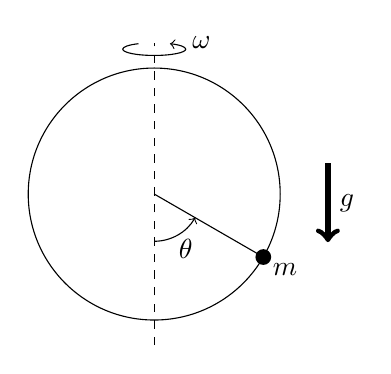
\begin{tikzpicture}[scale=0.8]
    \def\rad{2}
    \def\ang{-30}
    \draw (0,0) circle[radius=\rad];
    \draw[dashed] (0,-1.2*\rad) -- (0,1.2*\rad);
    \draw (0,0) -- (\ang:\rad);
    % \fill[fill=DarkRed] (\ang:\rad) circle[radius=0.125];
    \fill (\ang:\rad) circle[radius=0.125];
    \node at (\ang:1.2*\rad) {$m$};
    \draw[->] (-90:0.75) arc (-90:\ang:0.75);
    \node at (-90-\ang:1){$\theta$};
    \draw (0,1.1*\rad) arc[start angle=-90, end angle=-240, x radius=0.5, y
    radius=0.1];
    \draw[->] (0,1.1*\rad) arc[start angle=-90, end angle=60, x radius=0.5, y
    radius=0.1];
    \node at (0.75,1.2*\rad){$\omega$};
    % \draw[accel, line width=2] (10:1.4*\rad) -- node[anchor=west]{$g$}
    \draw[->, line width=2] (10:1.4*\rad) -- node[anchor=west]{$g$}
    ++(0,-1.25);
  \end{tikzpicture}
  \end{center}

\end{problem}

\begin{solution}
  \vfill
\end{solution}
\newpage

\end{document}
